\documentclass[a4paper,11pt]{article}
\usepackage[margin=1in]{geometry}
\usepackage{graphicx}
\usepackage{caption}
\usepackage{subcaption}
\usepackage{parskip}
\usepackage{amsmath}

\makeatletter
\setlength{\@fptop}{5pt}
\makeatother

\title{Substitution Matrix Generation and Hidden Markov Model Statistical Parameter Estimation.}
\author{
Jacob Friedberg \\
\texttt{frie2142@vandals.uidaho.edu}
\and
Garrett Wells \\
\texttt{well1157@vandals.uidaho.edu}
}


\begin{document}
\maketitle
\begin{abstract}
    \noindent Substitution matrices are important tools in the bio-informatics toolkit. They allow researchers to determine how similar two sequences are to one another. Hidden Markov models also provide a similar usefulness by allowing researchers to determine how much parts of sequences contribute to characteristics of a gene. Using a list of 200 sequences we generate a substitution matrix using log-odds and estimate parameters for a Hidden Markov Model. We provide a substitution matrix, emission probability table, and state transition table from the data. The methods employed here produced good results which we are moderately confident in their accuracy. However, due to the small dateset size we are not confident that the substitution matrix or HMM parameters can be used generally on all types of sequences.
\end{abstract}

\section{Introduction}

In bio-informatics one of the crucial tools used to determine how similar two sequences are is a substitution or scoring matrix. These matrices give us a score when aligning sequences that can give us an idea of how related one sequence is to another. Two sequences are aligned with each other and character by character a score is accumulated across the sequence. There are several commonly used substitution matrices including BLOSUM-50, BLOSUM-62, and PAM. To generate these matrices, it is typical to calculate the log-odds score for each cell of the matrix. This score is created by analyzing the frequency at which a pair of characters appears in a large data set of sequences compared to the background frequency of each character and taking the $\log$ of that value. A scaling factor is used to scale the values to the range of $[-10,10]$. 


Of similar importance in bio-informatics is modeling the probability of observing gene sequences which contribute to characteristics of interest in a species. Such a model may then be used to analyze new gene samples to predict which characteristics they correspond to without employing the skills of a highly trained biologist. The model generated with this data is called a Hidden Markov Model(HMM) and uses the sequence of amino acids to predict the most probable state(genomic characteristic) that the sequence encodes for. The statistical information HMMs rely on is defined below:

\begin{description}
    \item[Emission] a symbol occurring(emitted) in a genome while in a specific state.
    \item[Transition] a change from one state to another, representing a change in the function or type of the sequence.
\end{description}

This information is then used to produce a state machine which relies on emissions and transitions to guide the model's state prediction. The algorithms used to calculate these key pieces of data and tables are described below.

In this paper we implement two algorithms: Generating a BLOSUM-like substitution matrix using a provided set of 200 sequences and calculating the emission and transition probabilities given a set of sequences that are annotated to indicate the locations where specific amino acids within the gene contribute to different characteristics of the \textit{Silacus Soulas} insect.


\section{Algorithm Descriptions}

\subsection{Substitution Matrix}

To generate a BLOSUM-like substitution matrix a log-odds score is used which is defined by equation \ref{eq:log-odds}.

\begin{equation}
	\label{eq:log-odds}
	{S_{(i,j)}} = {\frac{1}{\lambda}} \log \frac{P_{ij}}{F_i F_j}
\end{equation}

\begin{equation}
	\label{eq:scaling factor}
	{\frac{1}{\lambda}} = \text{Scaling factor}
\end{equation}

\begin{equation}
	\label{eq:prob-pairs}
	{P_{ij}} = \frac{\text{Number of i,j and j,i character pairs in all sequences}}{\text{Total pairs possible in all sequences}}
\end{equation}

\begin{equation}
	\label{eq:prob-frequencyi}
	{F_{i}} = \frac{\text{Occurrence of character i in all sequences}} {\text{Total number of characters in all sequences}}
\end{equation}

\begin{equation}
	\label{eq:prob-frequencyj}
	{F_{j}} = \frac{\text{Occurrence of character j in all sequences}} {\text{Total number of characters in all sequences}}
\end{equation}


A score for a pair of amino acid characters i and j is defined as the a scaling factor $\frac{1}{\lambda}$ multiplied by the log of the probability of an i,j character pair over the background frequency of i and j. To calculate ${P_{ij}}$, all sequences are aligned with each other and a column by column analysis takes place. For each column the number of i,j and j,i pairs are accumulated and divided by the total number of pairs possible for all sequences.  ${F_{j}}$ and ${F_{i}}$ are calculated by counting the occurrences of the characters divided by the total number of characters amongst all sequences. A scaling factor of $\lambda = 0.16 \text{ or } 6.25 \text{ times was used for our algorithm.}$

While devising the algorithm for implementing a log-odds score two key mathematical shortcuts were found. First, if we analyze the pattern of possible pairs created by moving down a 4 sequence list of length 1 as seen in Figure \ref{fig:screenshot001}, we can see something interesting. 

\begin{figure}[h]
	\centering
	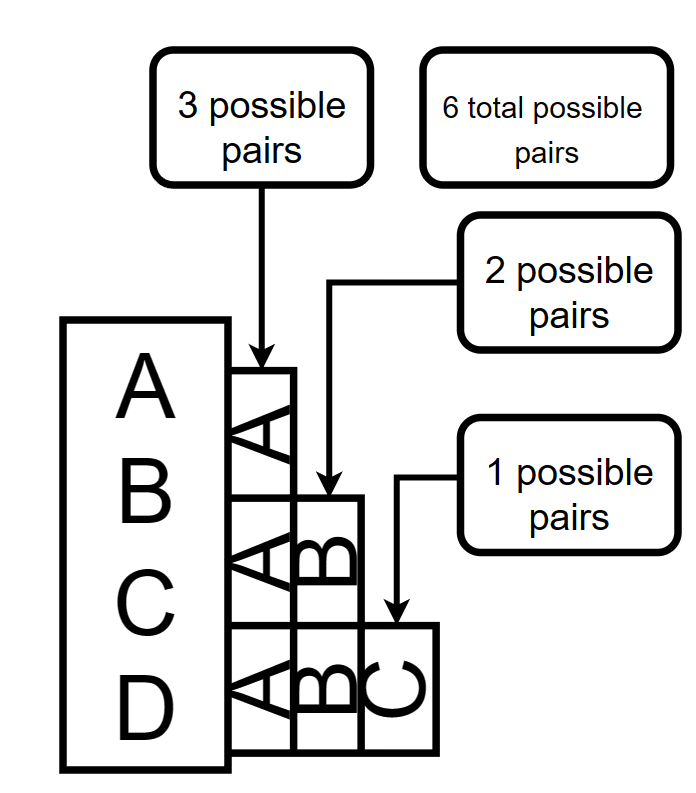
\includegraphics[width=0.25\linewidth]{screenshot001}
	\caption{}
	\label{fig:screenshot001}
\end{figure}

The number of total possible pairs in a given column is characterized by summation $\sum_{k=1}^{n-1} a_k$ where n is the number of sequences in the column. The closed form of this summation is:

\begin{equation}
	\label{eq:closed form}
	{\text{Total number of pairs in a column} = \sum_{k=1}^{n-1} a_k} =\frac{n^{2} + n}{2}
\end{equation}

The second shortcut was recognizing that since we are finding both i,j and j,i pairs, we can calculate the number of these pairs based purely on how many i and j characters are in a given column. 


\begin{equation}
	\label{eq:ij pairs}
	{\text{i,j and j,i pairs in column}} = \text{count of j in col} * \text{count of i in col}
\end{equation}

However, there is a limitation in the use of equation \ref{eq:ij pairs} as it can only be used for i,j pairs that are not the same character which would occur along the diagonal of our substitution matrix. Instead, equation \ref{eq:closed form} can be used where n is the number of a's in a column for an ${P_{aa}}$ calculation.

Using these two equations we can reduce the time complexity of our program immensely instead of having to go through all possible pairs of a column for the entire length of all the sequences which would incur a $K * \frac{n^{2} + n}{2}$ complexity where $K$ is the length of our sequences and $n$ is the number of sequences we have. We can reduce that down to just  $K * n$ by using equations \ref{eq:closed form} and \ref{eq:ij pairs} to determine how many pairs should exist based on the counts of characters we are interested in rather than manually indexing all sequences in a column and finding the pairs manually through comparison.






\subsection{Emission and Transition Probabilities}

As introduced in the definition for emission, a symbol refers to one of the 20 amino acids, represented by its single letter substitute. Examples can be seen in emission table \ref{emissions}. In the emission parameters are calculated individually for each symbol based on state. The equation used for these calculations is listed below. The term, $e_{s_{x}symbol_y}$, represents the number of occurrences of $symbol_y$ in state $s_x$. This term is divided by all occurrences of any symbol in state $s_x$ to produce a probability of seeing $symbol_y$ in $s_x$.

\begin{equation}
    \frac{e_{s_{x}symbol_y}}{\sum_{k=1}^n e_{s_xsymbol_k}}
\end{equation}


Transition parameters are described as the probability of ``transitioning from state \verb+X+ to state \verb+Y+''(see table \ref{transitions}). They are calculated as the number of observed transitions between two states, $s_x$ and $s_y$, divided by all observed transitions out of state $s_x$. Transitions between the symbols in the same state are counted to estimate the probability of remaining in the current state. The equation for this calculation is more formally stated below with $t$ representing observed transitions between two states.

\begin{equation}
    \frac{t_{s_{x}s_{y}}}{\sum_{k = 0}^{n} t_{s_{x}s_{k}}}
\end{equation}

As may be expected, all probabilities sum to 1, though in slightly different ways for each table. For the emission table, all probabilities for symbols seen in state \verb+0+(seen as one column of the table), for example will sum to 1. For the transition table, however, one horizontal row should be expected to sum to 1. Also note that though some transition probabilities are 0, this is considered acceptable since it is this represents that some segments of genome do not occur following others.

\section{Results}

\begin{table}[!hbp]
	\centering
	\begin{tabular}{l|*{20}{r} }
		& a  & r  & n & d & c & q  & e  & g  & h & i  & l  & k  & m  & f  & p  & s  & t & w & y  & v \\ \hline
		a & 7  & -1 & 1 & 3 & 2 & -1 & -1 & -2 & 1 & -2 & -2 & -1 & -1 & -2 & -1 & -2 & 3 & 1 & -1 & 1 \\
		r & -1 & 4  & 2 & 1 & 1 & 1  & 2  & 1  & 2 & 1  & 1  & 2  & 3  & 2  & 2  & 2  & 1 & 1 & 1  & 1 \\
		n & 1  & 2  & 4 & 1 & 1 & 2  & 2  & 1  & 2 & 2  & 1  & 1  & 2  & 1  & 3  & 1  & 2 & 1 & 1  & 2 \\
		d & 3  & 1  & 1 & 3 & 2 & 1  & 2  & 2  & 2 & 2  & 1  & 2  & 1  & 2  & 1  & 2  & 2 & 1 & 1  & 2 \\
		c & 2  & 1  & 1 & 2 & 4 & 0  & 0  & 2  & 1 & 1  & 2  & 2  & 2  & 1  & 2  & 2  & 0 & 0 & 3  & 1 \\
		q & -1 & 1  & 2 & 1 & 0 & 4  & 1  & 0  & 2 & 2  & 3  & 1  & 2  & 2  & 1  & 1  & 2 & 1 & 1  & 0 \\
		e & -1 & 2  & 2 & 2 & 0 & 1  & 4  & 2  & 3 & 3  & 0  & 1  & 2  & 1  & 0  & 2  & 1 & 2 & 1  & 0 \\
		g & -2 & 1  & 1 & 2 & 2 & 0  & 2  & 4  & 1 & 2  & 2  & 1  & 1  & 2  & 2  & 3  & 1 & 2 & 0  & 1 \\
		h & 1  & 2  & 2 & 2 & 1 & 2  & 3  & 1  & 4 & 2  & 1  & 2  & 1  & 1  & 0  & 2  & 3 & 1 & 2  & 0 \\
		i & -2 & 1  & 2 & 2 & 1 & 2  & 3  & 2  & 2 & 3  & 1  & 2  & 3  & 3  & 2  & 2  & 1 & 1 & 1  & 0 \\
		l & -2 & 1  & 1 & 1 & 2 & 3  & 0  & 2  & 1 & 1  & 5  & 1  & 1  & 1  & 2  & 2  & 1 & 1 & 2  & 1 \\
		k & -1 & 2  & 1 & 2 & 2 & 1  & 1  & 1  & 2 & 2  & 1  & 3  & 1  & 0  & 2  & 1  & 3 & 2 & 2  & 1 \\
		m & -1 & 3  & 2 & 1 & 2 & 2  & 2  & 1  & 1 & 3  & 1  & 1  & 3  & 2  & 1  & 1  & 1 & 2 & 2  & 1 \\
		f & -2 & 2  & 1 & 2 & 1 & 2  & 1  & 2  & 1 & 3  & 1  & 0  & 2  & 3  & 2  & 1  & 1 & 1 & 1  & 1 \\
		p & -1 & 2  & 3 & 1 & 2 & 1  & 0  & 2  & 0 & 2  & 2  & 2  & 1  & 2  & 4  & 2  & 0 & 1 & 1  & 1 \\
		s & -2 & 2  & 1 & 2 & 2 & 1  & 2  & 3  & 2 & 2  & 2  & 1  & 1  & 1  & 2  & 3  & 2 & 1 & 1  & 2 \\
		t & 3  & 1  & 2 & 2 & 0 & 2  & 1  & 1  & 3 & 1  & 1  & 3  & 1  & 1  & 0  & 2  & 3 & 1 & 2  & 1 \\
		w & 1  & 1  & 1 & 1 & 0 & 1  & 2  & 2  & 1 & 1  & 1  & 2  & 2  & 1  & 1  & 1  & 1 & 3 & 0  & 2 \\
		y & -1 & 1  & 1 & 1 & 3 & 1  & 1  & 0  & 2 & 1  & 2  & 2  & 2  & 1  & 1  & 1  & 2 & 0 & 4  & 1 \\
		v & 1  & 1  & 2 & 2 & 1 & 0  & 0  & 1  & 0 & 0  & 1  & 1  & 1  & 1  & 1  & 2  & 1 & 2 & 1  & 4\\
		\hline
	\end{tabular}
	\caption{Generated BLOSUM-like scoring matrix}
    \label{substitutions}
\end{table}

\begin{table}[!hbp]
    \centering
    \caption{Emission Percentage By State}
    \vspace{0.5cm}
    \begin{tabular}{|c|c  c  c|}
        \hline
        \textbf{Amino Acid} & \multicolumn{3}{|c|}{\textbf{State}} \\
        \hline
        -  &  0 & 1 & 2 \\
        \hline
        a & 3.91 & 7.94 & 1.59 \\
        \hline
        c & 3.84 & 2.75 & 6.86 \\
        \hline
        d & 1.87 & 1.72 & 4.18 \\
        \hline
        e & 3.91 & 2.62 & 5.62 \\
        \hline
        f & 6.60 & 4.96 & 5.55 \\
        \hline
        g & 3.73 & 1.85 & 4.86 \\
        \hline
        h & 3.65 & 1.77 & 3.63 \\
        \hline
        i & 2.91 & 2.13 & 5.01 \\
        \hline
        k & 3.29 & 2.40 & 4.96 \\
        \hline
        l & 3.48 & 5.26 & 4.22 \\
        \hline
        m & 4.67 & 4.28 & 4.79 \\
        \hline
        n & 5.58 & 2.35 & 5.41 \\
        \hline
        p & 5.84 & 3.71 & 5.75 \\
        \hline
        q & 5.44 & 2.18 & 5.38 \\
        \hline
        r & 2.82 & 1.75 & 5.18 \\
        \hline
        s & 5.77 & 4.17 & 4.90 \\
        \hline
        t & 5.96 & 11.10 & 5.75 \\
        \hline
        v & 11.35 & 14.54 & 5.38 \\
        \hline
        w & 7.43 & 11.86 & 6.43 \\
        \hline
        y & 7.97 & 10.66 & 4.56 \\
        \hline
    \end{tabular}
    \label{emissions}
\end{table}


\begin{table}[!ht]
    \centering
    \caption{Transitions Percentage Between States }
    \vspace{0.5cm}
    \begin{tabular}{|c|c c c|}
        \hline
        \textbf{From State} & \multicolumn{3}{c|}{\textbf{To State}} \\
        \hline
        - & 0 & 1 & 2 \\
        \hline
        0 & 96.1 & 3.89 & 0.00 \\
        1 & 0.00 & 92.01 & 7.99 \\
        2 & 1.54 & 0.00 & 98.5 \\
        \hline
    \end{tabular}
    \label{transitions}
\end{table}

\end{document}
